\subsection{Arquitectura}


El sistema sigue una arquitectura orientada a servicios, donde existe un único servicio llamado \textit{Core Service} 
que se estructura como monolito modular (para su fácil extracción a servicios independientes), accesible a través 
de un \textit{API Gateway} que actúa como punto de entrada único, proporcionando terminación TLS y enrutamiento de 
solicitudes. 

\vspace{0.25cm}

El sistema cuenta con dos aplicaciones web: la \textit{Landing Page}, orientada a presentar el producto al público general, 
y el \textit{Back Office}, destinado a la administración interna del sistema. Por otro lado, el Cliente de Juego permite 
a los usuarios conectarse y jugar en cualquier mundo disponible, y el Editor de Mundos está destinado a la 
creación y modificación de mundos.

\vspace{0.25cm}

El Core Service coordina la comunicación entre estos clientes, el clúster de mundos y los sistemas de 
almacenamiento, que comprenden una base de datos relacional (PostgreSQL) para recursos del \textit{Core Service}, 
una base de datos no relacional (MongoDB)  para la persistencia del estado de los jugadores, y 
dos buckets de archivos para assets cosméticos y contenido general de los mundos.

\vspace{0.25cm}

El entorno de juego se distribuye en un clúster de instancias de zona escalables, donde cada zona activa se ejecuta 
como una instancia independiente que admite conexiones directas de jugadores. El despliegue dinámico de estas 
instancias es gestionado por el Core Service mediante Nomad. Por último, la observabilidad del sistema se delega 
a Datadog, que centraliza métricas, logs y alertas de los distintos componentes de forma continua.

\begin{figure}[H]
  \centering
  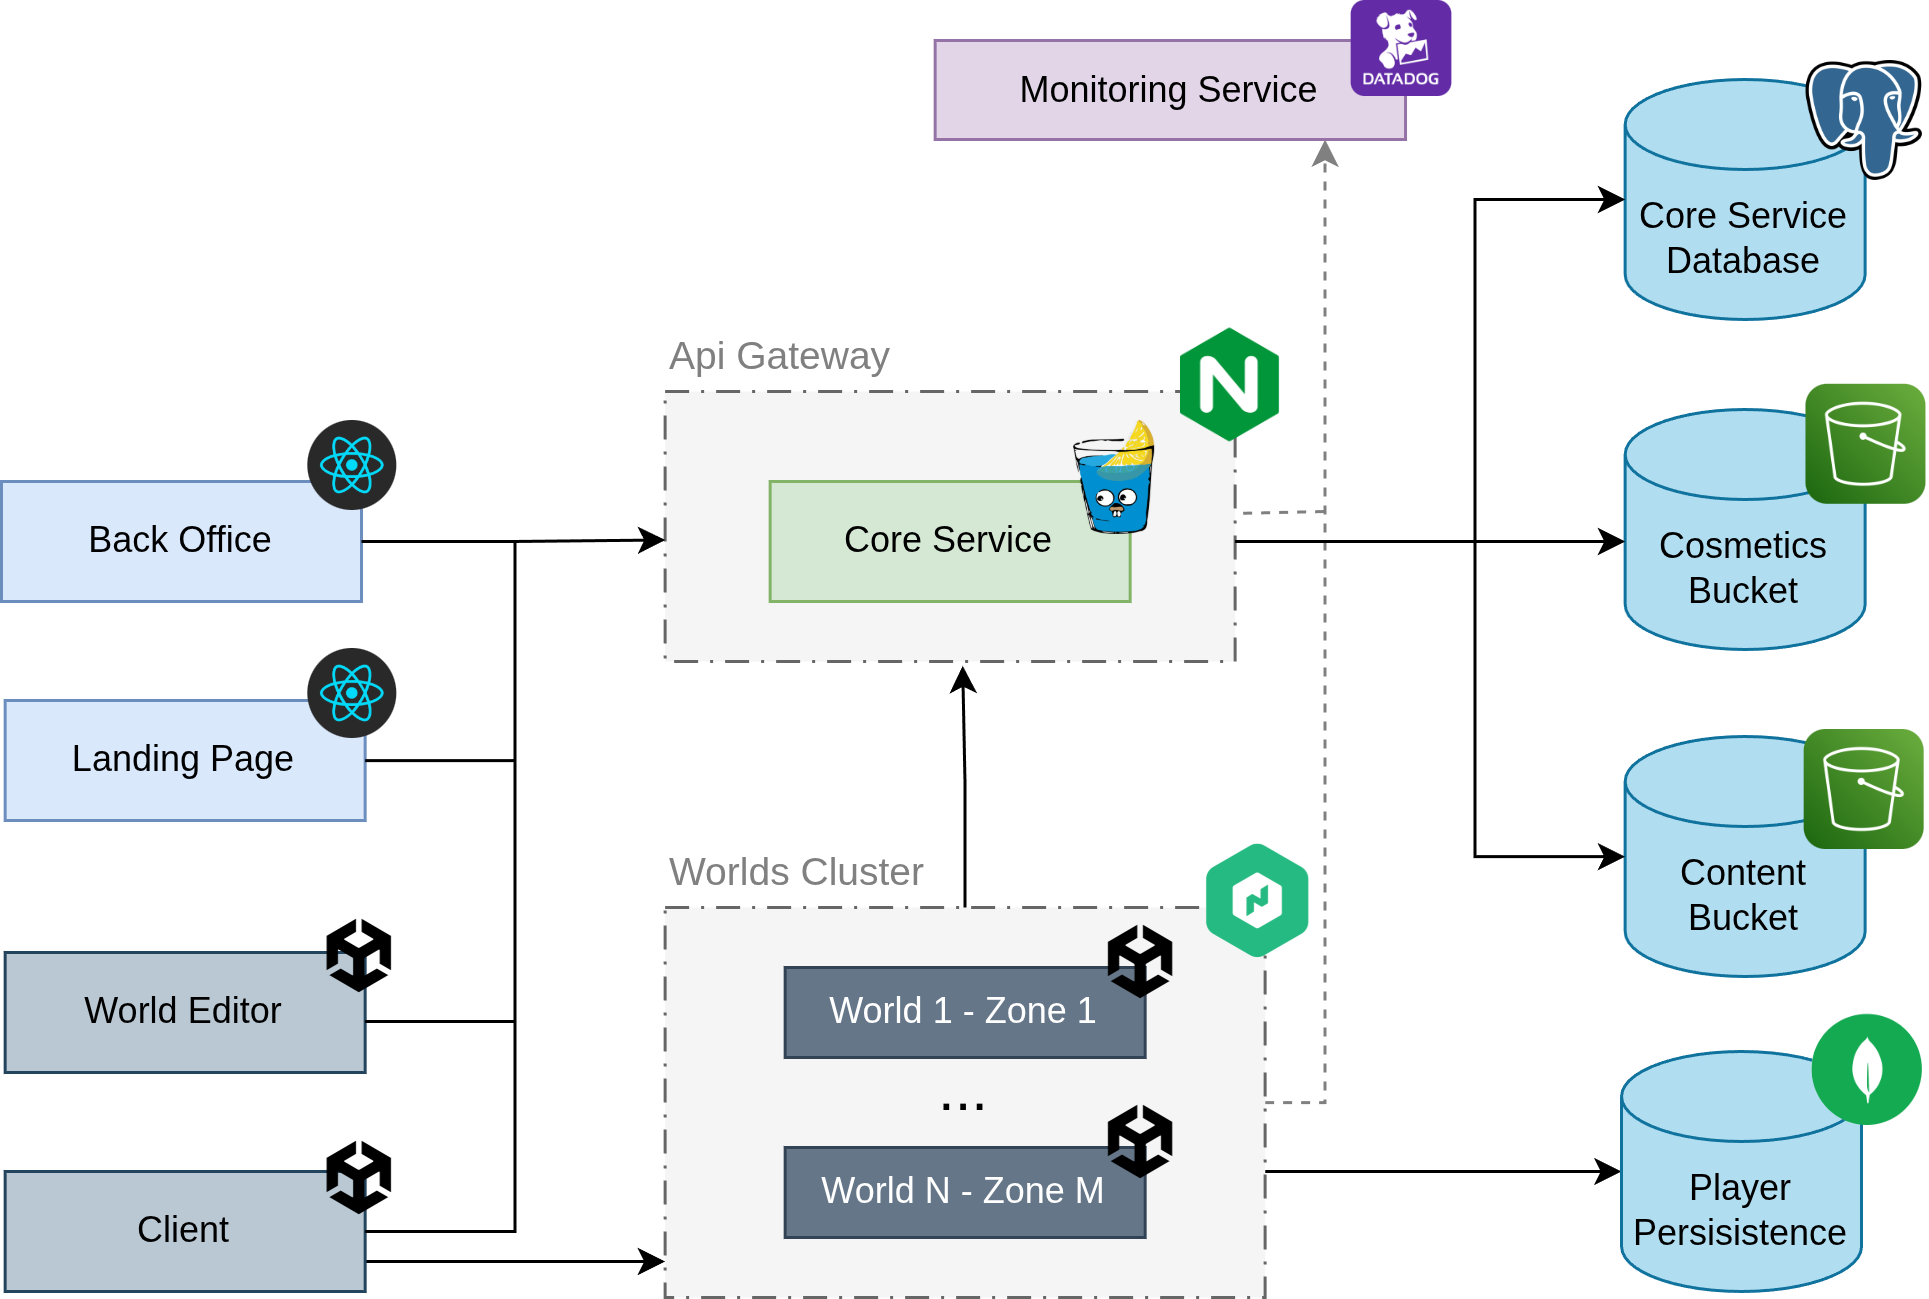
\includegraphics[width=\textwidth]{img/08-implemented-solution/architecture.png}
  \caption{Diagrama de arquitectura del sistema}
  \label{fig:architecture}
\end{figure}